\section{Integrated multi-crop stochastic model}

Let crops be indexed by $i=1,\ldots,n$ and let $x_i$ denote acreage. Random per-acre profit is $\widetilde\pi_i=\widetilde p_i\widetilde y_i-c_i$, where price and yield may be dependent within and across crops and baseline cost $c_i$ is deterministic. Portfolio profit and loss are
\begin{equation}
\Pi(x,\omega)=\sum_i x_i\widetilde\pi_i(\omega),\qquad L(x,\omega)=-\Pi(x,\omega).
\end{equation}
Returns are linear in acreage. Fixed setup costs, endogenous prices, crop interactions and multi-period state variables are outside the baseline and would require a different feasible set or objective.

Operational feasibility is represented by the non-empty polytope
\begin{equation}
X=\{x\in\R^n:\ell\leq x\leq u,\;\mathbf 1^\top x\leq A,\;c^\top x\leq B,\;Gx\leq g\}.
\label{eq:feasible}
\end{equation}
The rows of $Gx\leq g$ accommodate rotation, contract, agronomic and other shared restrictions. Land is an inequality because idling can be optimal or forced; full use requires an admissible profitable expansion. In the experiments these constraints are controlled interventions. They are not estimates of private farm restrictions.

For confidence level $\alpha\in(0,1)$, loss-CVaR is
\begin{equation}
r_\alpha(x)=\cvar_\alpha[L(x)]=\min_{v\in\R}\left\{v+\frac{1}{1-\alpha}\E[(L(x)-v)_+]\right\}.
\label{eq:cvar}
\end{equation}
The canonical problem maximizes expected profit $\mu^\top x$, where $\mu_i=\E[\widetilde\pi_i]$, subject to $x\in X$ and $r_\alpha(x)\leq\kappa$. The sign convention protects against large losses. For finite scenarios $s$ with positive weights $w_s$, a free $v$ and non-negative excess-loss variables $q_s$ yield a linear programme.

Marginal profit distributions $F_i$ and a valid $n$-copula $C_\theta$ define the joint law. Pairwise lower-tail dependence is a diagnostic when its limit exists, but does not identify a copula, a conditional tail mean or an allocation. Named Gaussian, Student-$t$, Clayton and empirical-copula laws are therefore compared as complete scenario-generating models, never as if a single scalar ordered all portfolio losses \citep{demarta2005tcopula,ansari2024dependence}.

A suitability vector $s$ induces a weak order, with ties forming equivalence classes. Proportional and winner-take-all rules are benchmark mappings, not optima by definition. Let
\begin{equation}
S_\kappa=\arg\max\{\mu^\top x:x\in X,\;r_\alpha(x)\leq\kappa\}.
\end{equation}
For a strict pair $s_i>s_j$ and tolerance $\tau_x$, reversal at $x$ means $x_j-x_i>\tau_x$. It is \emph{possible} if this holds at some $x\in S_\kappa$, \emph{universal} if it holds at every $x\in S_\kappa$, and \emph{selected} if it holds for a declared deterministic selection. Strong and top-rank reversal add zero-allocation and highest-tie-class conditions. This set-valued vocabulary separates properties of the decision problem from properties of one solver-returned vertex.

Figure~\ref{fig:geometry} locates four exact two-crop cases in the same acreage simplex. An expected-margin case reverses the external score because cardinal profit margins point elsewhere. Operational bounds can place the entire feasible set in the reversal half-space. A binding risk limit can move the optimal point without implying monotone crop-wise comparative statics. A flat optimal face can contain both reversing and non-reversing points, so selected reversal depends on the selection rule even though possible and universal reversal remain well defined.

\begin{figure}[t]
\centering
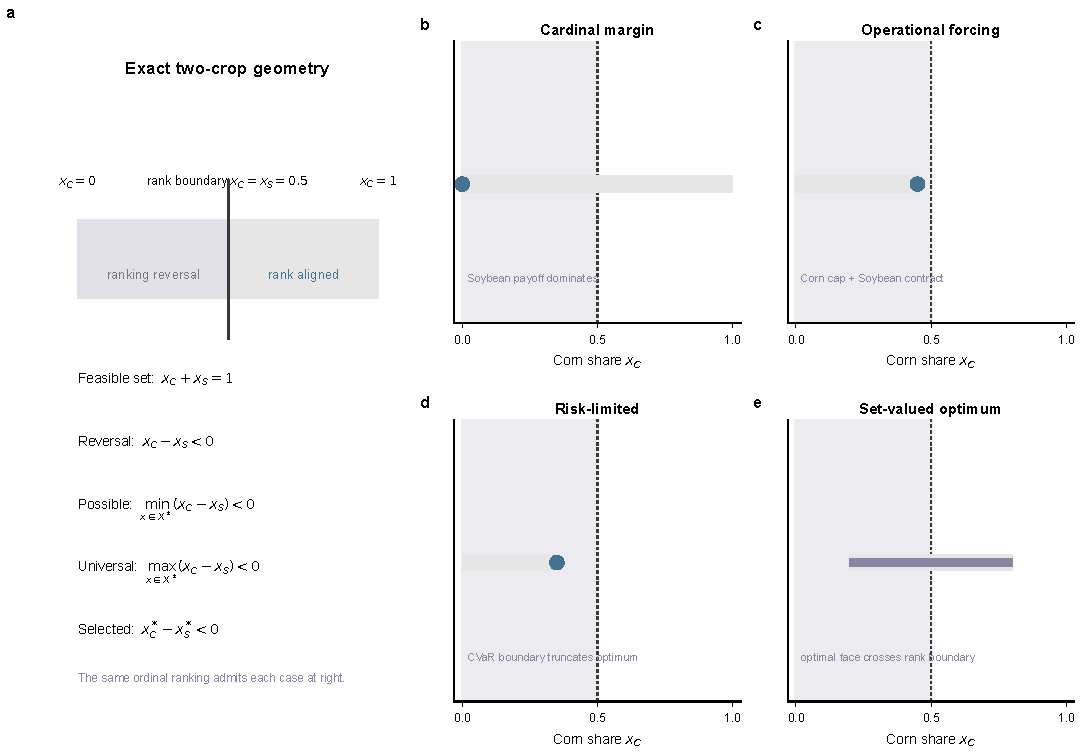
\includegraphics[width=\textwidth]{../figures/stage_ii/main/Figure2.pdf}
\caption{\textbf{Exact geometry of distinct ranking-reversal mechanisms.} Two-crop constructions distinguish cardinal-margin, operational, risk-limited and set-valued mechanisms. Shading marks the corn--soybean reversal half-space. The cases are analytic constructions, not empirical estimates.}
\label{fig:geometry}
\end{figure}
